
\documentclass{report}

\usepackage[utf8]{inputenc}
\usepackage[italian]{babel}
\usepackage{import}
\usepackage{todonotes}
\usepackage{color}
\usepackage{rotating}
\usepackage[hidelinks]{hyperref}
\usepackage{url}
\usepackage{pdfpages}
\usepackage{siunitx}
\usepackage{pdflscape}
\usepackage{subfig}
\usepackage[euler]{textgreek}
\usepackage{mhchem}

\usepackage{enumerate} 
\usepackage{amsmath}
\usepackage{amsfonts}

\usepackage[signatures,swapnames,sans]{frontespizio}

\usepackage{geometry}
\geometry{portrait, margin=3cm}
\usepackage{siunitx}
\usepackage{booktabs}

\renewcommand*\figurename{Figura}

\newcommand{\sub}[1]{\textsubscript{#1}}
\newcommand{\super}[1]{\textsuperscript{#1}}
\newcommand{\parallelsum}{\mathbin{\!/\mkern-5mu/\!}}

\newcommand{\Fig}[0]{Fig.}

\usepackage{titlesec}

\titleformat{\chapter}{\normalfont\huge}{}{20pt}{\huge\bfseries}

\linespread{1.1}

\begin{document}
	\begin{frontespizio}
		\Margini{3cm}{3cm}{3cm}{3cm}
		\Universita{Bergamo}
		\Logo[43.332mm]{unibg-mark}
		\Divisione{Scuola di Ingegneria}
		\Corso[Laurea Magistrale]{Ingegneria Informatica}
		\Titolo{Laboratorio di Elettronica}
		\Sottotitolo{Relazione esperienza di laboratorio 1}
		\Punteggiatura{}
		\NRelatore{Prof.}{Prof.}
		\Relatore{Luigi Gaioni}
		\Candidato[1058231]{Giulia Allievi}
		\Candidato[1059640]{Martina Fanton}
		\Annoaccademico{2022--2023}
		\begin{Preambolo*}
			\usepackage[italian]{babel}
			\usepackage[T1]{fontenc}
			\usepackage[utf8]{inputenc}
			\usepackage{microtype}
			\usepackage{lmodern}
			\graphicspath{{img/}}
			
			\renewcommand{\frontinstitutionfont}{\fontsize{14}{17}\bfseries\scshape}
			\renewcommand{\fronttitlefont}{\fontsize{17}{21}\bfseries\scshape}
			\renewcommand{\frontfootfont}{\fontsize{12}{14}\bfseries\scshape}
		\end{Preambolo*}
	\end{frontespizio}

%----------------------------------------------------------------------------------------
%	PAGINA BIANCA
%----------------------------------------------------------------------------------------
\newpage
\null
\thispagestyle{empty}
\newpage

%----------------------------------------------------------------------------------------
%	INTRO
%----------------------------------------------------------------------------------------
\chapter{Filtro passa-basso attivo}
\section{Introduzione}
% circuito da realizzare
% uA741
% spiegazione veloce pin
Il primo circuito che abbiamo realizzato è un filtro passa-basso attivo. Questo circuito per funzionare ha bisogno di un amplificatore operazionale, che è un dispositivo... . Per il nostro circuito abbiamo utilizzato un amplificatore operazionale \textit{general purpose}, il \textmu A741. Nell'immagine sottostante, la figura \ref{figura:741}, si possono vedere i numeri e la funzione di ogni terminale di questo componente. \par
\begin{figure}[h]
\centering
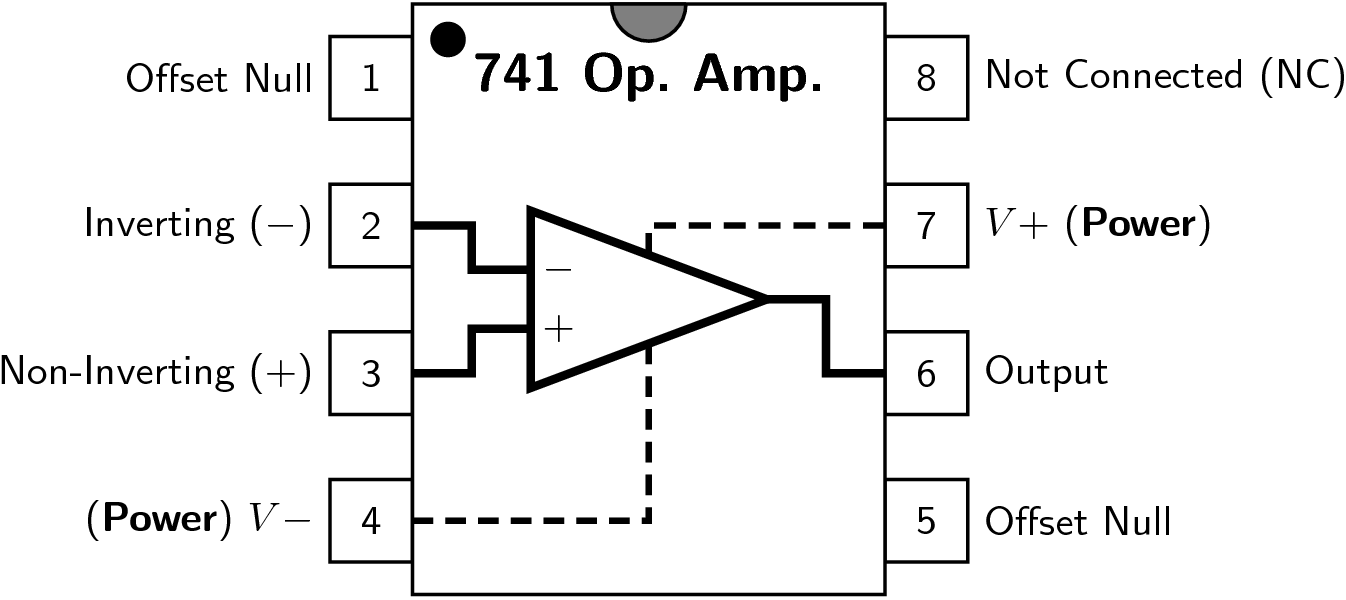
\includegraphics[height=5.5cm]{immagini/741pinout}
\caption{Package e funzione dei pin del \textmu A741.}
\label{figura:741}
\end{figure}

\newpage % da togliere a sezione precedente terminata
\section{Schema del circuito e analisi teorica}
Lo schema del circuito è riportato in figura \ref{figura:cto_filtro}. Dato che l'amplificatore operazionale è un circuito attivo, per funzionare correttamente deve essere alimentato. Abbiamo utilizzato un'alimentazione duale, con tensione positiva di \SI{10}{\volt} e alimentazione negativa di \SI{-10}{\volt}. è duale perché non c'è un'alimentazione pari alla massa. \par % sistemare
\begin{figure}[h]
\centering
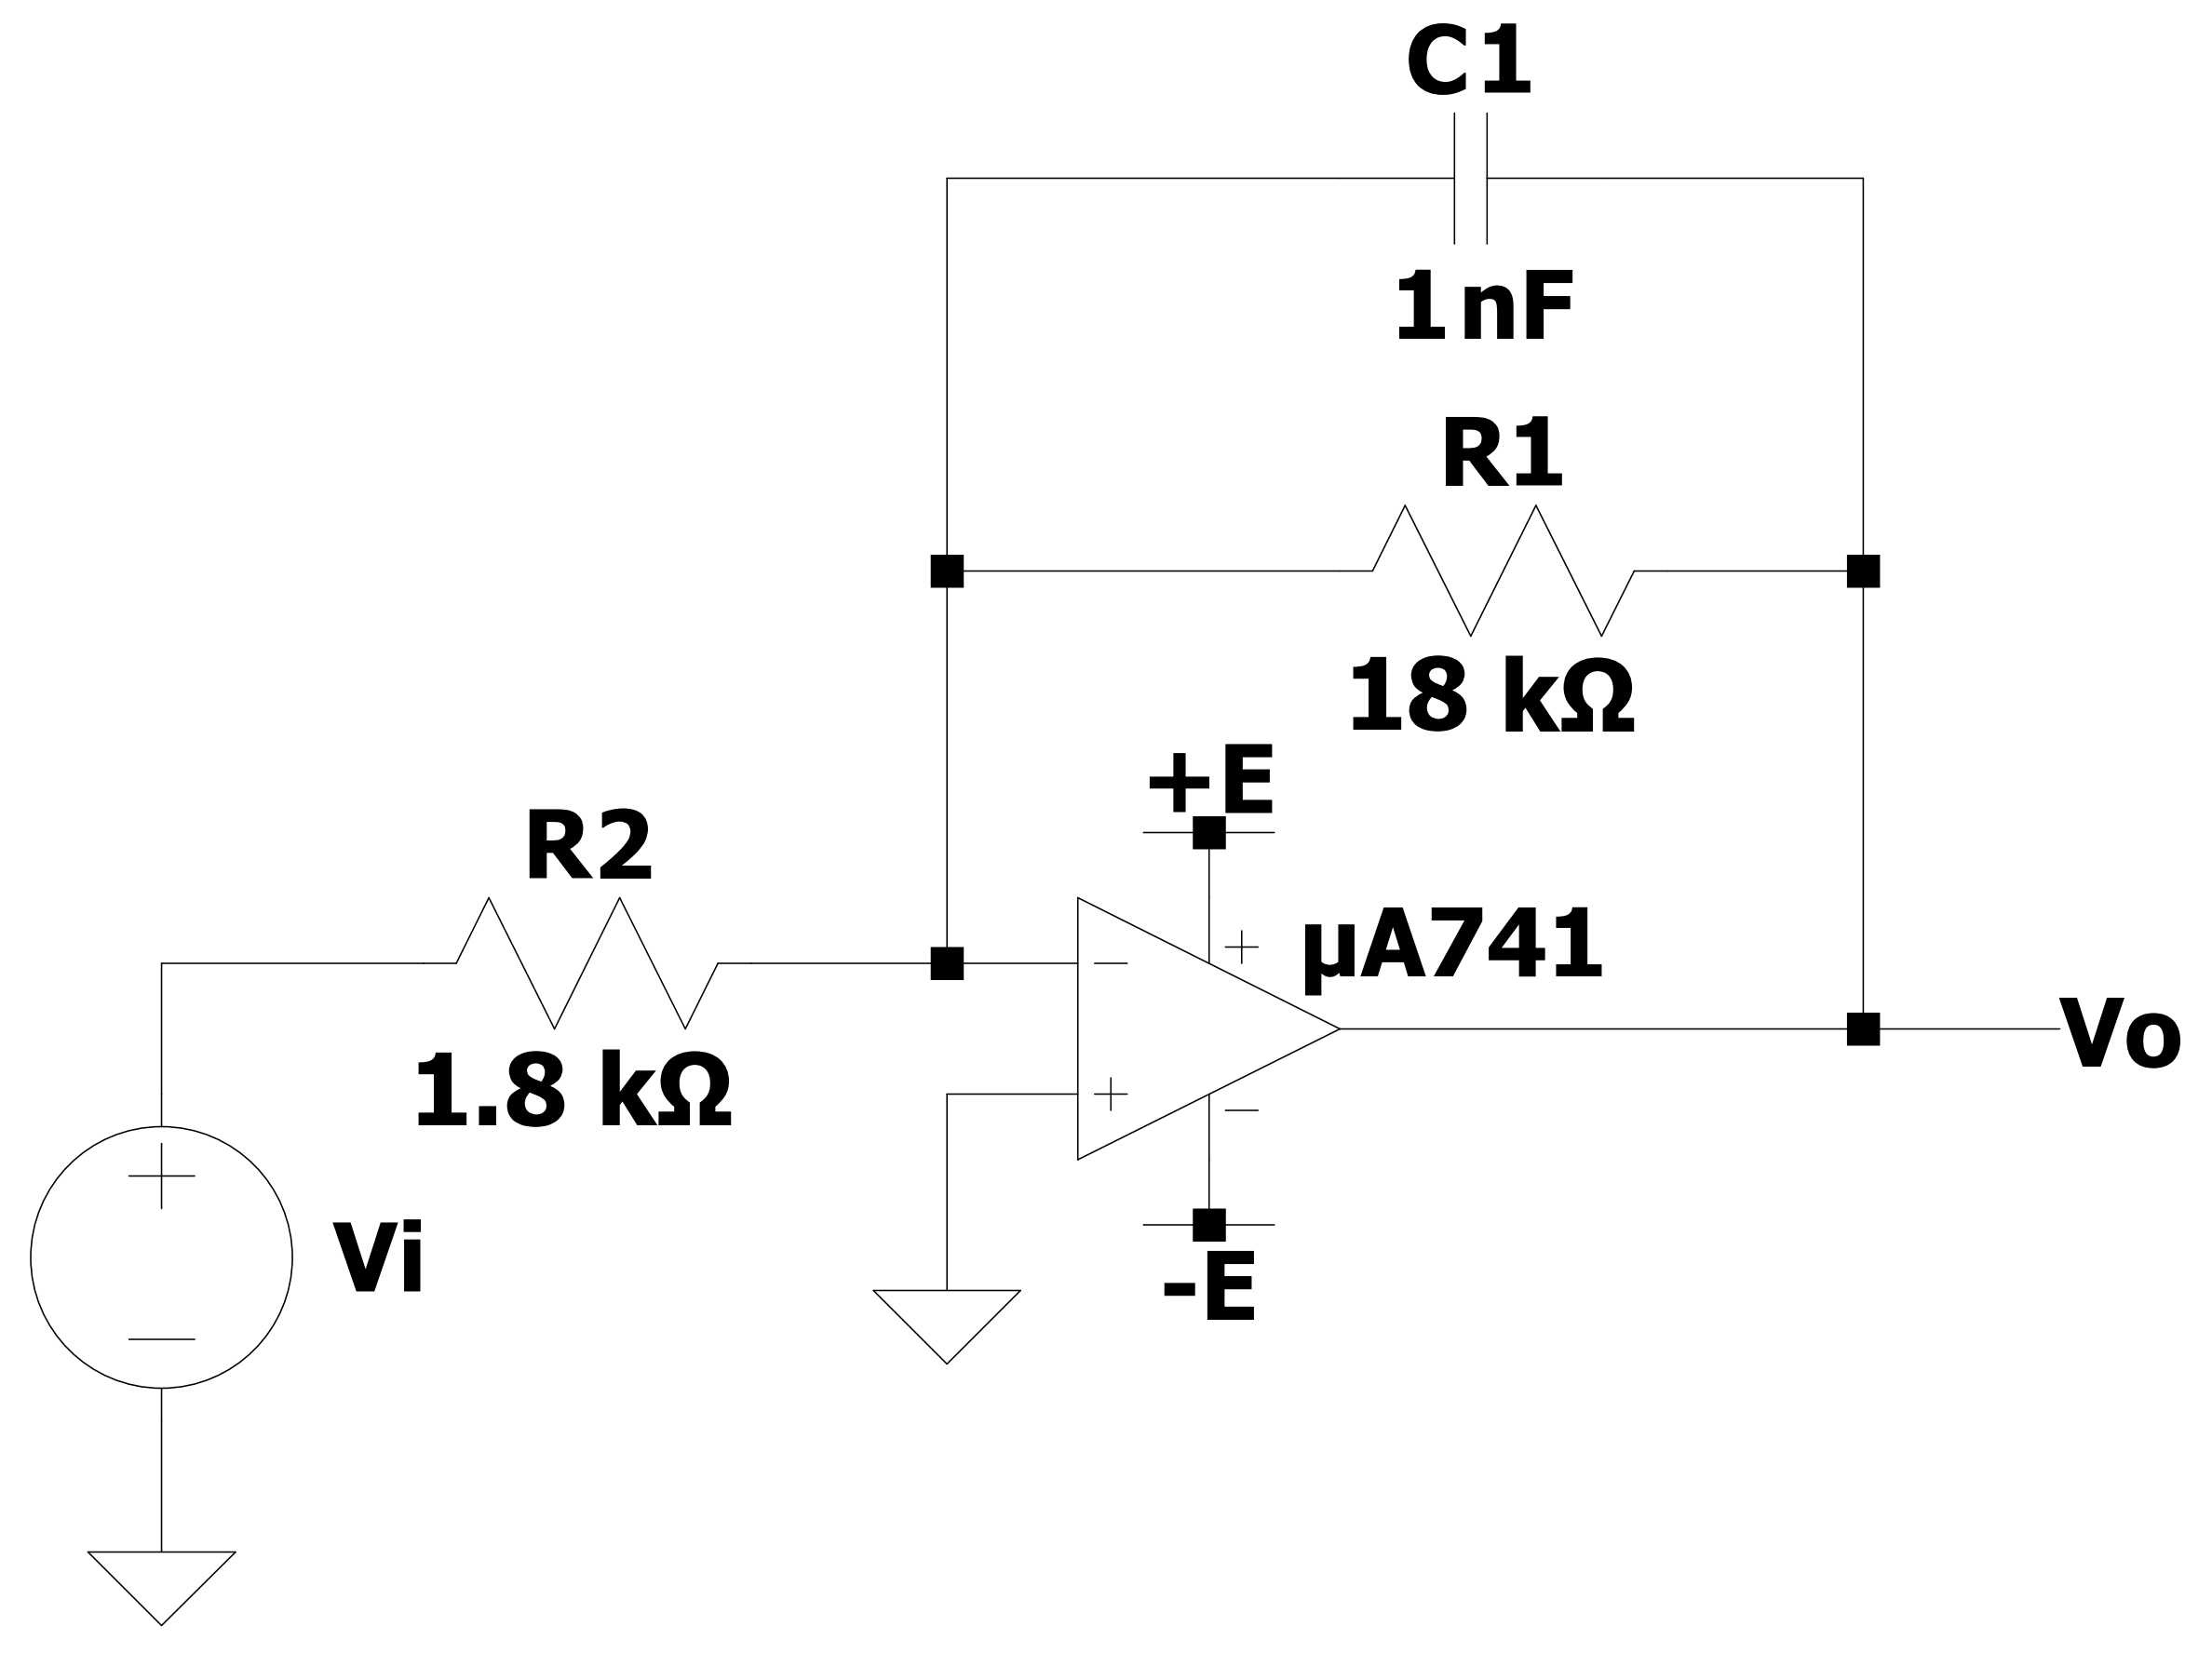
\includegraphics[height=9cm]{immagini/cto_filtro}
\caption{Schema dell'amplificatore invertente.}
\label{figura:cto_filtro}
\end{figure}
%% Analisi (da EMI)
\noindent Per analizzare questo circuito facciamo riferimento alla figura \ref{figura:cto_analisi}.
\begin{figure}[h]
\centering
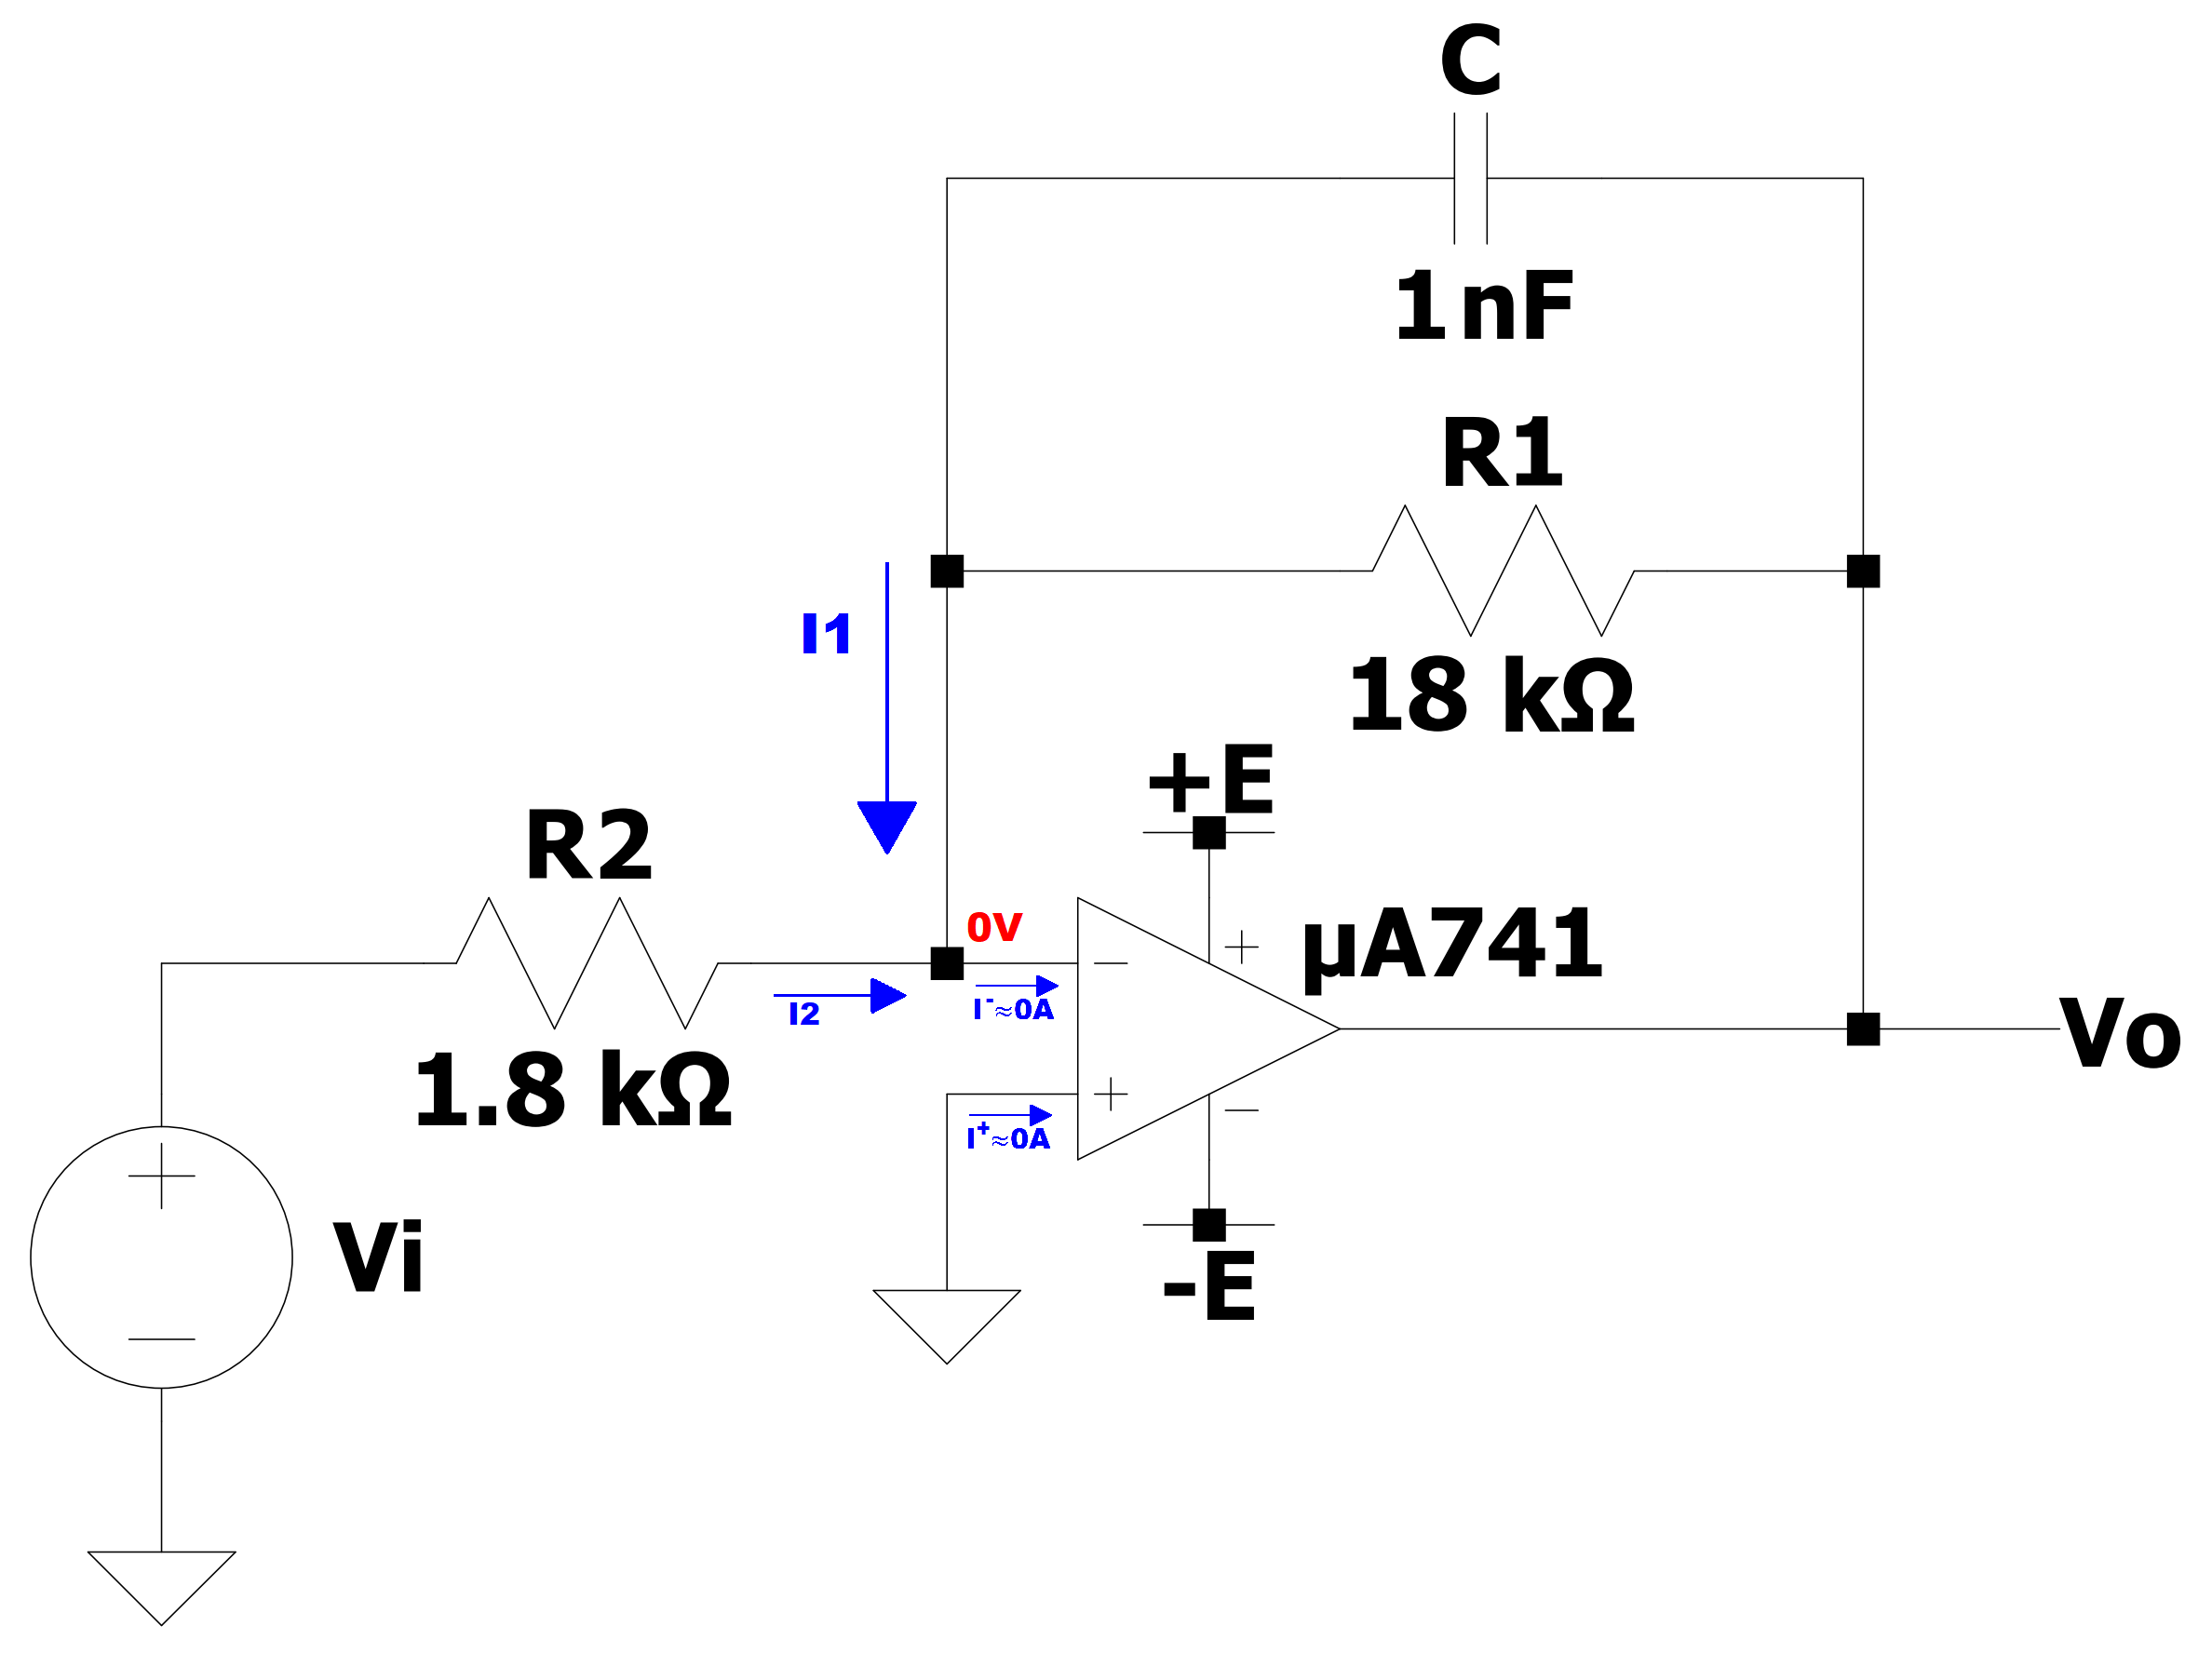
\includegraphics[height=9cm]{immagini/cto_filtro_analisi}
\caption{Schema per analizzare l'amplificatore invertente.}
\label{figura:cto_analisi}
\end{figure}
La resistenza $R_1$ e il condensatore $C_1$ sono in parallelo, pertanto si può calcolare l'impedenza equivalente:
\\[2pt]\indent$\displaystyle{Z_{eq}=C_1\parallelsum R_1=\frac{\frac{1}{s\cdot C_1} \cdot R_1}{\frac{1}{s\cdot C_1} + R_1}=\frac{\frac{R_1}{s\cdot C_1}}{\frac{1+s\cdot R_1C_1}{s\cdot C_1}}=\frac{R_1}{1+s\cdot R_1C_1}}$
\\Per ricavare la funzione di trasferimento del circuito è sufficiente fare un bilancio di correnti all'ingresso invertente. Con $I_1$ si intende la corrente che scorre nell'impedenza equivalente $Z_{eq}$.
\\[2pt]\indent $I_2=I_1+I^-$
\\[2pt]La corrente in ingresso all'OPAMP è molto piccola, idealmente $I^+=I^-\rightarrow 0A$. Perciò l'equazione precedente diventa:
\\\indent $\displaystyle{I_2=I_1}$
\\Utilizzando la legge di Ohm generalizzata, le correnti si possono esprimere come:
\\[2pt]\indent $\displaystyle{\frac{V^-(s)-V_i(s)}{R_2}=(V_o(s)-V^-(s))\cdot\frac{1+s\cdot R_1C_1}{R_1}}$
\\[2pt]Se un circuito è retroazionato negativamente, $V^+=V^-$ per il principio del cortocircuito virtuale. Dato che $V^+$ è a massa, la sua tensione è di 0V, di conseguenza anche $V^-$ si troverà a questa tensione. L'equzione precedente diventa:
\\[2pt]\indent $\displaystyle{\frac{-V_i(s)}{R_2}=V_o(s)\cdot\frac{1+s\cdot R_1C_1}{R_1}}$
\\[2pt]Tramite quest'equazione è facile ricavare la funzione di trasferimento del circuito, che risulta:
\\[2pt]\indent $\displaystyle{\frac{V_o(s)}{V_i(s)}=-\frac{R_1}{R_2}\cdot\frac{1}{1+s\cdot R_1C_1}}$
\\[2pt]La funzione di trasferimento ottenuta è quella di un filtro passa-basso, perché al denominatore troviamo il termine $1+s\cdot R_1C_1$. Vediamo che c'è però anche un fattore di guadagno pari al rapporto fra $R_1$ e $R_2$. Compare anche un segno meno, pertanto l'ingresso e l'uscita saranno sfasate di 180°
\\Se passiamo al regime sinusoidale, sostituiamo $s$ con $j\omega$. La funzione di trasferimento diventa:
\\[2pt]\indent $\displaystyle{\frac{V_o(\omega)}{V_i(\omega)}=-\frac{R_1}{R_2}\cdot\frac{1}{1+j\omega\cdot R_1C_1}}$
%% se lav a freq basse, espr si semplifica

\newpage % da togliere a sezione precedente terminata
\section{Misure e osservazioni}
% dimensionamento + misure componenti usati
% connessioni 
% foto
% oscilloscopio
% tabella (c'è già)
% matlab
% considerazioni teo vs sper
% saturazione
% offset

\begin{table}[h]
	\centering
	\begin{tabular}{|c|c|c|c|c|}
		\hline
		\textbf{Frequenza} &\boldmath$\displaystyle\mathrm{{V_{PP,in}}}$ \textbf{[V]} & \boldmath$\displaystyle\mathrm{{V_{PP,out}}}$\textbf{[V]} & \textbf{Guadagno} & \textbf{Sfasamento [°]}\\
		\hline
		100 Hz & 0.488 & 4.804 & 9.84 & -179.3\\
		\hline
		500 Hz & 0.488 & 4.799 & 9.83 & -176.8\\
		\hline
		1 kHz & 0.485 & 4.779 & 9.85 & -173.4\\
		\hline
		5 kHz & 0.481 & 4.188 & 8.71 & -149.7\\
		\hline
		8.8 kHz & 0.484 & 3.388 & 7.00 & -133.9\\
		\hline
		10 kHz & 0.485 & 3.163 & 6.52 & -129.7\\
		\hline
		50 kHz & 0.483 & 0.833 & 1.72 & -96.3\\
		\hline
		100 kHz & 0.484 & 0.427 & 0.88 & -87.7\\
		\hline
		500 kHz & 0.487 & 0.943 & 1.94 & -58.6\\
		\hline
		1 MHz & 0.488 & 0.542 & 1.11 & -41.9\\
		\hline
		5 MHz & 0.477 & 0.621 & 1.30 & -35.9\\
		\hline
		10 MHz & 0.430 & 0.106 & 0.25 & -9.8\\
		\hline\end{tabular}
\caption{Grandezze misurate ad ongi frequenza.}
\label{table:misure}
\end{table}


%----------------------------------------------------------------------------------------

\end{document}
